%from scipy.stats import beta, norm, gamma
%from numpy import linspace, average, std
%x = linspace(0.0, 0.06)
%beta_x = beta.pdf(x, 2.462049740861992, 29.502013726920467, 0.0005845381630033533, 0.20813302210781293)
%norm_x = norm.pdf(x, 0.016615628892405383, 0.009681441990708757)
%gamma_x = gamma.pdf(x, 2.7500499267384706, 0.0003644996765732702, 0.005909429918741313)
%beta_mean = beta.mean(2.462049740861992, 29.502013726920467, 0.0005845381630033533, 0.20813302210781293)
%norm_mean = norm.mean(0.016615628892405383, 0.009681441990708757)
%gamma_mean = gamma.mean(2.7500499267384706, 0.0003644996765732702, 0.005909429918741313)
%print(f'Beta Mean: {beta_mean}\nNorm Mean: {norm_mean}\nGamma Mean: {gamma_mean}\n')
%print(f'Average: {average([beta_mean, norm_mean, gamma_mean])}')
%print(f'STD: {std([beta_mean, norm_mean, gamma_mean])}')
%
%print('\\addplot [very thick, blue!50!black] coordinates {')
%for i in list(zip(x, beta_x)):
%    print(f'\t({i[0]}, {i[1]})')
%
%print('};')
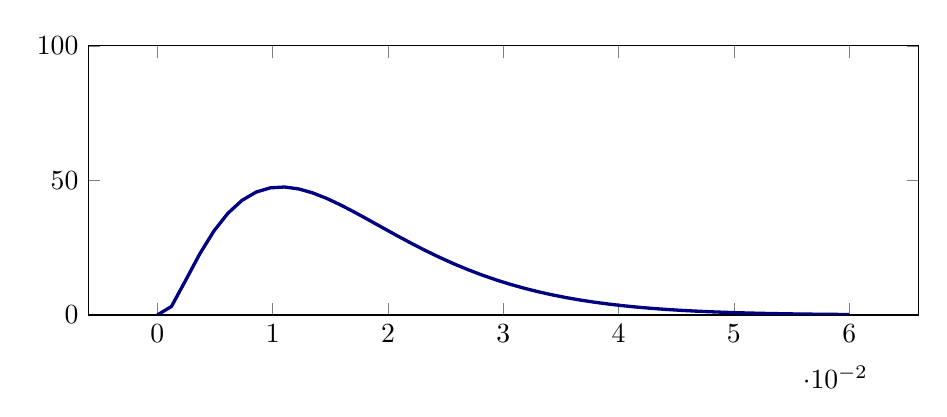
\begin{tikzpicture}
    \begin{axis}[try min ticks=3, ymin=0, ymax=100,width=\linewidth, height=5cm,
        log ticks with fixed point]
        \addplot [very thick,blue!50!black] coordinates {
            (0.0, 0.0)
            (0.0012244897959183673, 3.185370433486203)
            (0.0024489795918367346, 12.849116233840686)
            (0.003673469387755102, 22.68508457236311)
            (0.004897959183673469, 31.161253710289554)
            (0.006122448979591836, 37.81753339019626)
            (0.007346938775510204, 42.608051910362846)
            (0.00857142857142857, 45.673546807801884)
            (0.009795918367346938, 47.235848966364564)
            (0.011020408163265306, 47.543261462563336)
            (0.012244897959183673, 46.84128896346183)
            (0.01346938775510204, 45.357261275791295)
            (0.014693877551020407, 43.29296827259877)
            (0.015918367346938776, 40.822011769104705)
            (0.01714285714285714, 38.08992329390769)
            (0.01836734693877551, 35.215851622648394)
            (0.019591836734693877, 32.29507317751616)
            (0.020816326530612245, 29.401856861684436)
            (0.022040816326530613, 26.59239242933872)
            (0.023265306122448978, 23.907606708272933)
            (0.024489795918367346, 21.375767433168306)
            (0.025714285714285714, 19.01482386260446)
            (0.02693877551020408, 16.834465434535016)
            (0.028163265306122447, 14.837900120588907)
            (0.029387755102040815, 13.023366635771918)
            (0.030612244897959183, 11.385401799256073)
            (0.03183673469387755, 9.91588787584037)
            (0.03306122448979592, 8.60490586919338)
            (0.03428571428571428, 7.4414203306201285)
            (0.03551020408163265, 6.413819877665804)
            (0.03673469387755102, 5.510335692046834)
            (0.037959183673469385, 4.71935806543318)
            (0.03918367346938775, 4.0296687732451515)
            (0.04040816326530612, 3.430604805269111)
            (0.04163265306122449, 2.912166846252753)
            (0.04285714285714286, 2.465083926187479)
            (0.044081632653061226, 2.080843872660651)
            (0.04530612244897959, 1.7516976048998794)
            (0.046530612244897955, 1.4706439089517072)
            (0.04775510204081632, 1.2314001171116706)
            (0.04897959183673469, 1.0283630694133308)
            (0.05020408163265306, 0.856563845615125)
            (0.05142857142857143, 0.7116190066923018)
            (0.052653061224489796, 0.5896804593163186)
            (0.05387755102040816, 0.48738553972437737)
            (0.055102040816326525, 0.40180849023321946)
            (0.05632653061224489, 0.3304141590851045)
            (0.05755102040816326, 0.2710144802527024)
            (0.05877551020408163, 0.22172807349347673)
            (0.06, 0.18094313682248273)
        };
    \end{axis}
\end{tikzpicture}